\chapter{Proposed System}

This chapter will present our proposed system as the solution. We will define our system and show how it solves the problem of maintaining privacy for the users. Then we will discuss about a generic prototype we made using the design from the proposed system. We will describe different parts of the system and how the end user perceives it.
\section{User Identification}
In order to solve the problem we first look at how the users are identified in the system. There are 2 ways by which a bank can identify the actual users
\begin{itemize}
	\item From the logs i.e. transaction data
	
The bank store all the logs or transaction data with real identity of the user. It is easy to access this data by the bank for a given user and extract all of his data.
	\item From a database in the bank system where personal details of the user are stored.	

The bank stores personal data about all its users in a database. As this database lies at the bank, it is possible for the bank to use the database to get the personal information about a user.
\end{itemize}
We can remove this identification in the following ways:
\begin{itemize}
	\item Remove the user identity from the logs and transaction data

Like this there is no way for the bank to get transaction data for a given user as there will be no user identity linked to the logs or transactions.
	\item Either remove the user's personal data or limit the access to this personal database.

If the bank removes the personal database of the users from its side, then there is no way the bank can get personal information of the users.

If the bank limits the access to such database and doesn't really use it for day to day banking purposes then it is also possible for the bank to limit access to the user's personal information.
\end{itemize}
\section{Pseudonym System}
In order to provide privacy to the users, we suggest a new pseudonym system as shown in figure \ref{fig:Pseudonym}.
\begin{figure}[h]
\centering
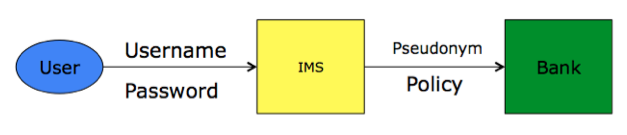
\includegraphics[width=\textwidth]{figures/Pseudonym}
\caption{Pseudonym Banking System}
\label{fig:Pseudonym}
\end{figure}
In our system we modify the Authentication service and replace it with an Identity Mapping System (IMS)"
\begin{itemize}
	\item Instead of giving the User ID to the bank we actually replace it with a pseudonym.
	\item The IMS sends the policy as well as the account ID to the bank.	
	\item The bank then uses this information to provide servicea to the customer.
	\item The bank doesn’t need to store the mapping databases.
\end{itemize}
The IMS can either be in the bank, in a separate department,it can be managed by a 3rd party. This way the bank doesn’t need to know the exact identity of the user to provide them with the services.
Also, the bank can still store personal details of the user in case of the legal requirement, but it can be stored at a separate place as it is not needed for day to day operation of the bank.
\section{Properties}
The privacy properties mentioned below are desirable in our pseudonym system:
\begin{itemize}
	\item \textbf{Unlinkability :} If the same pseudonym is used with different identities, or different pseudonyms are used for the same identity, it should not be possible to link these different transactions to the same person. 
	\item \textbf{Partial Information Disclosure :} The information given by a user should be minimum and he should be able to choose what information values he actually wants to be made available to the bank. 
	\item \textbf{Conditional Anonymity Removal :} In case of some discrepancy or legal requirement, the authorities should be able to come in and identify the real user from the Pseudonym.
	\item \textbf{Revocation :} It should be easy to revoke any user. Also, it should be easy to check whether a certain user is revoked or not. 
\end{itemize}
\section{User Privacy}
As in our system the bank never gets the real identity of the user, the user anonymity to the bank is maintained. Also bank doesn't need to store the policies for the users as its all coming from the IMS. As a result, it decreases a lot of load from the bank to store such data. IMS service adds a layer of pseudonymity in the system. 

\section{Generic Prototype}
Now we will talk about a generic prototype based on our proposed system 
For end user it doesn't change anything. End user authenticates to the IMS and then IMS creates a pseudonym for the user. This pseudonym is then used by the bank for providing the services to the customer.
\subsection{Authentication}
\begin{figure}[h]
	\centering
	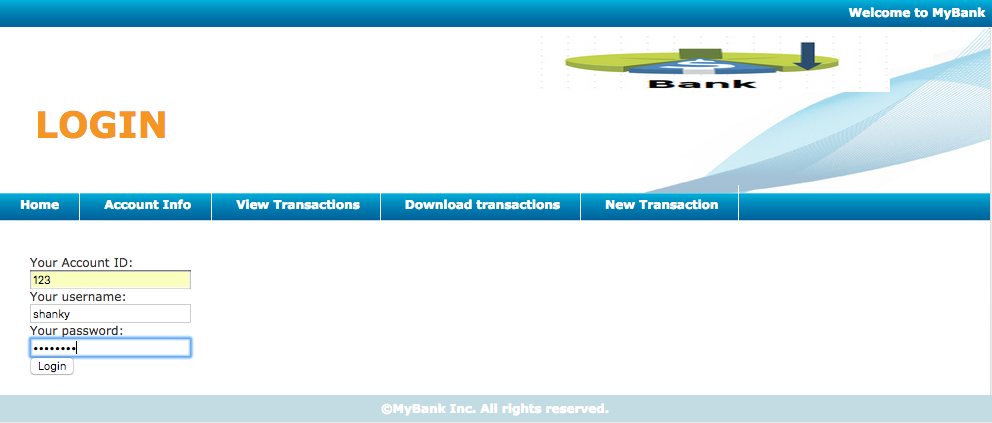
\includegraphics[width=\textwidth]{figures/Login}
	\caption{User Login Page}
	\label{fig:Login}
\end{figure}
\begin{figure}[h]
	\centering
	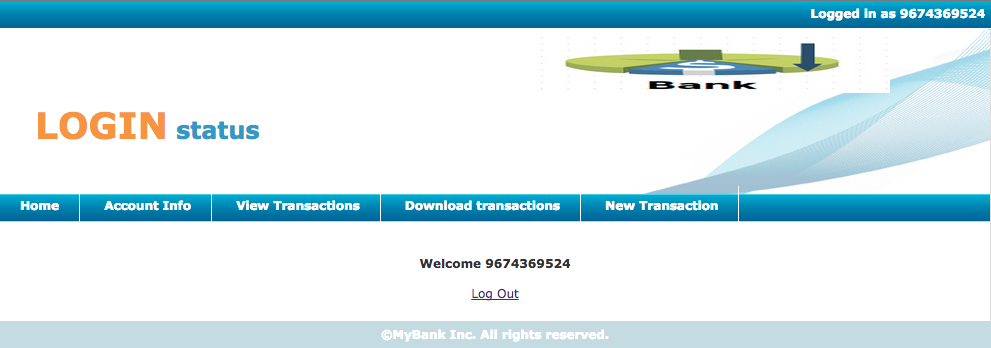
\includegraphics[width=\textwidth]{figures/Logged}
	\caption{Authenticated User}
	\label{fig:Logged}
\end{figure}	
User authentication happens as follows:
\begin{itemize}
	\item User goes to the bank login page.
	\item User puts his credentials in the login system.
	\item User credentials are verified by IMS and then user is redirected to his account page.
\end{itemize}
One thing to note that is that as traditional user, this doesn't change anything on the user end. User still use the same process to get access to his account.

As we can see in \ref{fig:Logged}, after authentication user is logged in with a pseudonym.	
\subsection{User Information}
\begin{figure}[h]
	\centering
	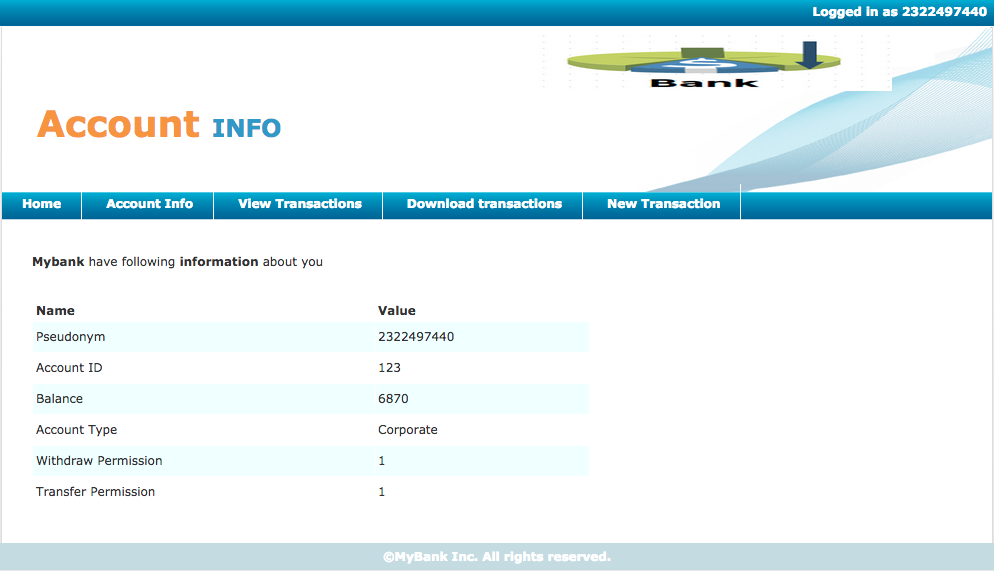
\includegraphics[width=\textwidth]{figures/Account1}
	\caption{User Information - Session 1}
	\label{fig:Account1}
\end{figure}	
\begin{figure}[h]
	\centering
	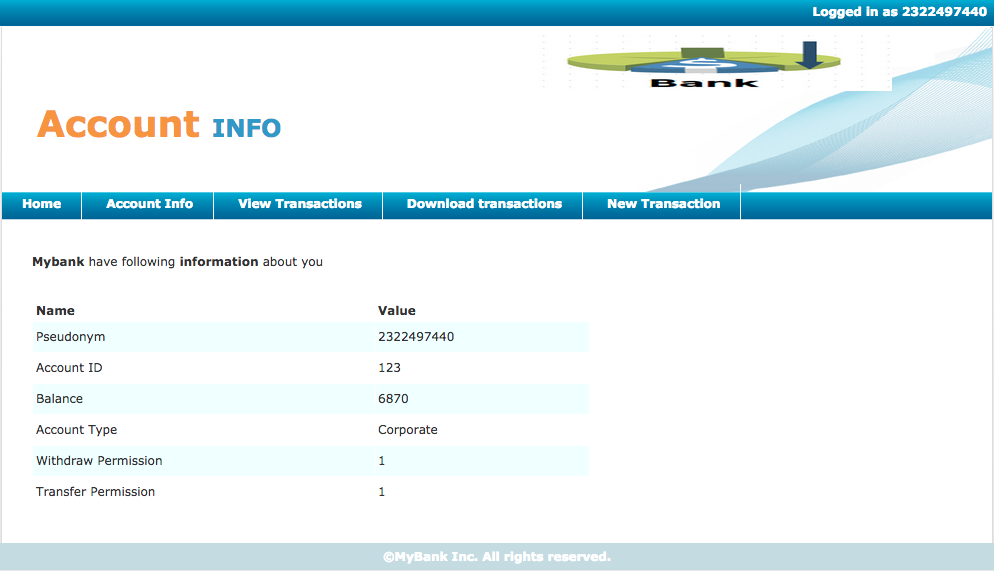
\includegraphics[width=\textwidth]{figures/Account1}
	\caption{User Information - Session 2}
	\label{fig:Account2}
\end{figure}
When we go to user information page we can see the information that is given to the bank by IMS for a given user.

In our case it is:
\begin{itemize}
	\item Pseudonym
	\item Account ID
	\item Balance
	\item Account Type
	\item Policies
	\begin{itemize}
		\item Withdraw Permission
		\item Transfer Permission
	\end{itemize}
\end{itemize}
As we can see from figure \ref{fig:Account1} and figure \ref{fig:Account2}, 2 different sessions of the same user are logged in with different pseudonym. Bank have no way to find out that its the same user who have logged into different sessions.

\subsection{Transactions}
\begin{figure}
	\centering
	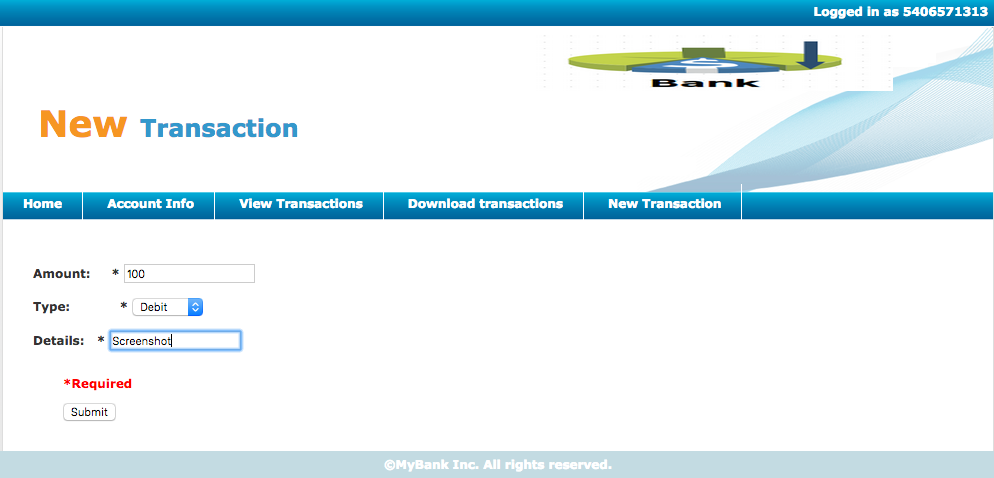
\includegraphics[width=\textwidth]{figures/New}
	\caption{New Transactions}
	\label{fig:New}
\end{figure}
In our prototype user is allowed to do 2 types of transactions
\begin{itemize}
	\item Debit
	\item Credit
\end{itemize}
All the transactions that are done by the user are logged in with the pseudonym; with which user has been logged in to the system.

Figure \ref{fig:New} shows the new transactions page in the system where user is allowed to do the transactions.
\begin{figure}[h]
	\centering
	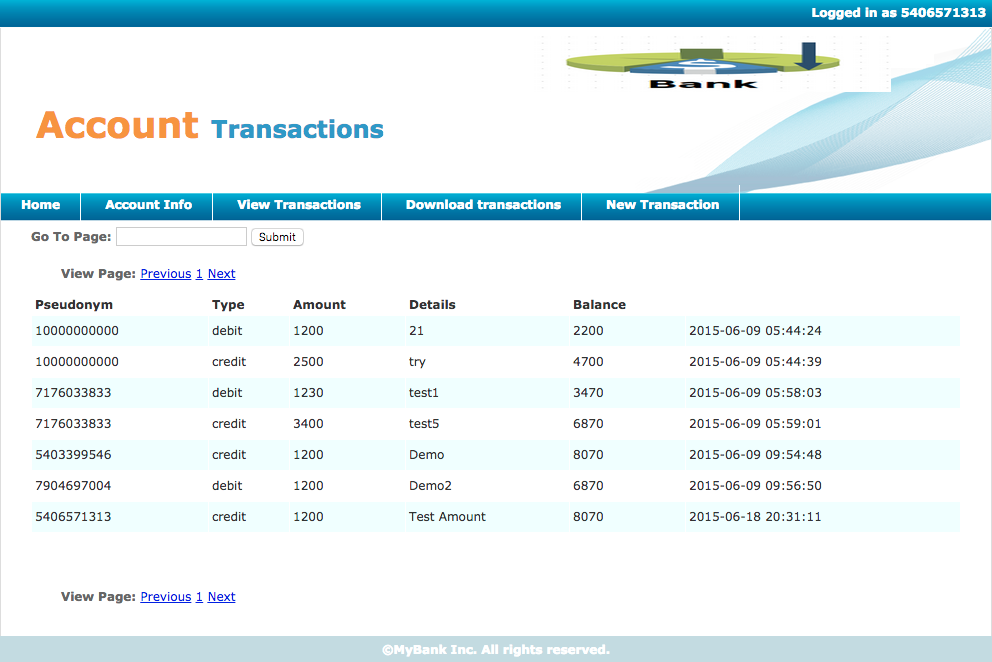
\includegraphics[width=\textwidth]{figures/Transactions}
	\caption{Account Transactions}
	\label{fig:Transactions}
\end{figure}

Figure \ref{fig:Transactions} shows all the transactions that has been done on the given account by users. As we can see, all the transactions are saved with the pseudonym of the users.
\begin{figure}[h]
	\centering
	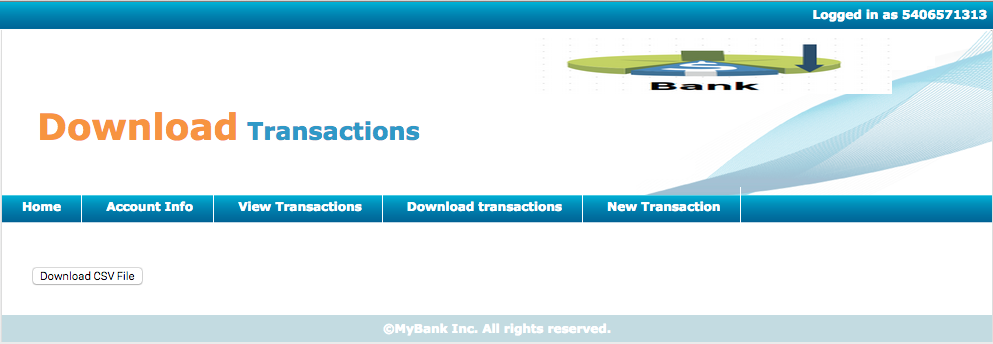
\includegraphics[width=\textwidth]{figures/Download}
	\caption{Download Transactions Option}
	\label{fig:Download}
\end{figure}
\begin{figure}[h]
	\centering
	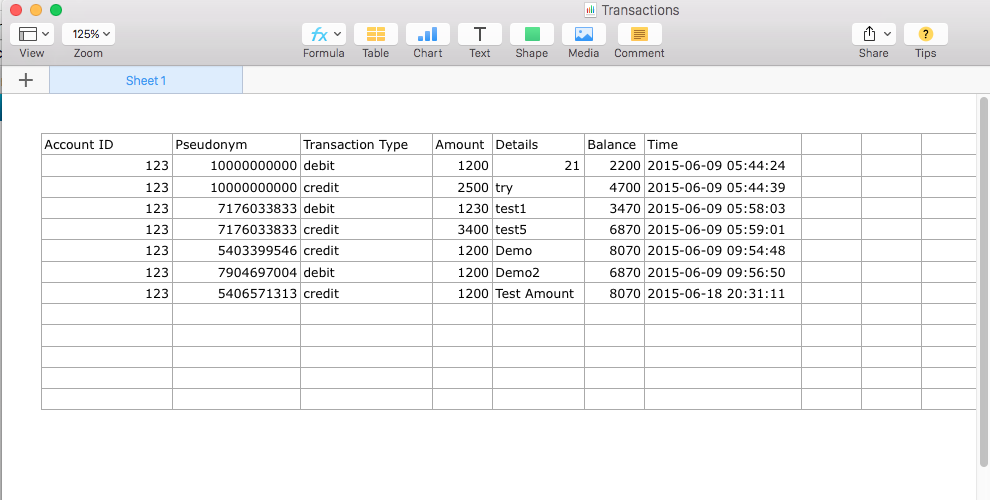
\includegraphics[width=\textwidth]{figures/File}
	\caption{Downloaded Transactions File}
	\label{fig:File}
\end{figure}	
Our system also allow the users to download the transactions from the download transactions page as shown in figure \ref{fig:Download}. These transactions are stored in a csv file and then can be seen as in figure \ref{fig:File}.
\FloatBarrier
In this chapter we presented our pseudonym system. Also we have given some certain privacy properties that our pseudonym system should be able to fulfill. Our generic system works with pseudonyms and in the next chapter we will talk about how we can replace our Identity Mapping System with OpenID and IDEMIX for our purposes

For our purposes we have decided to take case of 2 different systems for our IMS
\begin{itemize}
	\item OpenID
	\item IDEMIX
\end{itemize}.